\documentclass[8pt]{beamer}
\usetheme{default} % Very simple theme
\usecolortheme{dove} % Minimalist grayscale colors
\setbeamertemplate{navigation symbols}{} % Remove navigation bar

% Define brand-like colors
\definecolor{myblue}{RGB}{0, 102, 204}    % Blue for standard blocks
\definecolor{mygreen}{RGB}{0, 153, 0}     % Green for example blocks
\definecolor{myred}{RGB}{204, 0, 0}       % Red for alert blocks
\definecolor{myorange}{RGB}{255, 128, 0} % For \emph

% Accent color for titles, bullets, etc.
\setbeamercolor{structure}{fg=myblue}

% Block colors
\setbeamercolor{block title}{bg=myblue, fg=white}
\setbeamercolor{block body}{bg=blue!5, fg=black}

\setbeamercolor{exampleblock title}{bg=mygreen, fg=white}
\setbeamercolor{exampleblock body}{bg=green!5, fg=black}

\setbeamercolor{alertblock title}{bg=myred, fg=white}
\setbeamercolor{alertblock body}{bg=red!5, fg=black}
\setbeamercolor{alerted text}{fg=myred}

% Optional: color for \example text
\setbeamercolor{example text}{fg=mygreen}

% Custom emph (orange text instead of italic)
\let\oldemph\emph
\renewcommand{\emph}[1]{\textcolor{myorange}{#1}}


\usepackage{graphicx} % Package for images
\usepackage{amsmath} % Package for images
\graphicspath{{figs/}} % Path to your figures directory
\usepackage{array}  % For better column spacing
\usepackage{caption} % Required for \captionof

% Title Information
\title{STOCHASTIC METHODS IN WATER RESOURCES}
\vspace{25pt}
\subtitle{Unit 3: Random functions \\ Lecture 10: Spectral representation of random functions} 
\author{Luis Alejandro Morales, Ph.D.}
\institute{Universidad Nacional de Colombia \\ Department of Civil and Agriculture Engineering} %// }
%\date{\today}

\begin{document}

% Title Slide
\begin{frame}
    \titlepage
\end{frame}

%-------
% From Bierke
\section{Spectral representation of random functions}
\begin{frame}{Spectral representation of random functions: Definitions}
    \begin{itemize}
    \item \emph{Correlation functions} of a \emph{time series}, when analyzed for a longer period exhibit a \emph{periodic behaviour} e.g. \emph{Hole effect model} (see tables in lecture 9).
    \item For instance, the figures below show a time series of daily average streamflows and its \emph{correlation function}.

\begin{minipage}[l]{0.46\textwidth}
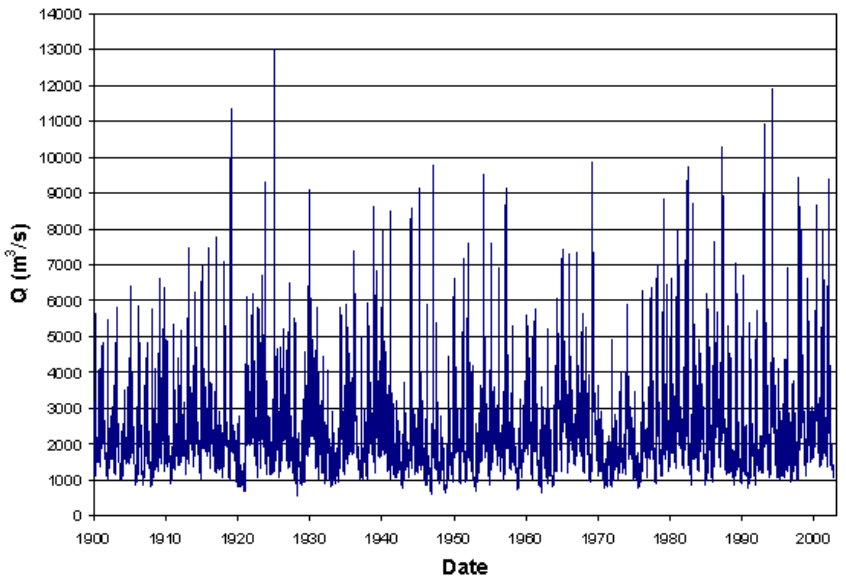
\includegraphics[width=\linewidth]{fiBi41.png}  % from Bierk
\end{minipage}
\hfill
\begin{minipage}[l]{0.46\textwidth}
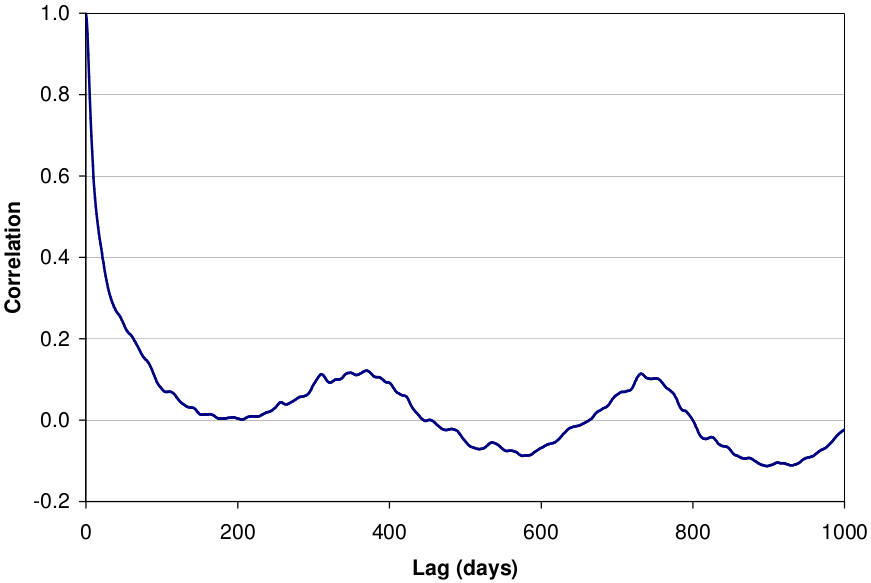
\includegraphics[width=\linewidth]{fiBi59.png}  % from Bierk
\end{minipage}
\item A clear periodic behaviour is observed in the \emph{correlation function} which is also apparent in the time series. 
\item Such periodicity is  caused because evaporation, which is driven by radiation and temperature, has a clear seasonal character, specially, at higher and lower latitudes and temperate climates. 
\item In conclusion, most hydrological time series show a \emph{seasonal variation}. This means that to analyse these models with \emph{stationary random functions} requires that \emph{seasonality} must be \emph{removed}.
\item The occurrence of \emph{seasonality } has also triggered the use of \alert{spectral methods} in stochastic modelling, although it must be stressed that spectral methods are also very suitable for analysing \emph{stationary random functions}.
    \end{itemize}
\end{frame}

\begin{frame}{Spectral density function}
    The \emph{spectral representation} of a \emph{stationary random function} $Z(t)$, means that $Z(t)$ is composed by the sum of its mean $\mu_Z$ and $2K$ \alert{sinosoids} with \emph{increasing frequencies}, where each frequency  has a \alert{random amplitude} $C_K$ and a \alert{random phase angle} $\Phi_K$. So $Z(t)$ is expressed as
    \vspace{-14pt}
    \[
        Z(t) = \mu_Z + \sum_{k = -K}^K C_K \cos(\omega_K t + \Phi_K)
    \]
    where $C_K = C_{-K}$, $\Phi_K = \Phi_{-K}$ and $\omega_K = \pm \frac{1}{2} (2k-1) \Delta \omega$.

The figure below is a schematic representation of the spectral decomposition of a stationary random function. The random signal is decomposed into its harmonics of increasing frequency ($\omega_K$) with random amplitude $C_K$ and random phase angle $\Phi_K$.
    \vspace{-2pt}
    \begin{center}
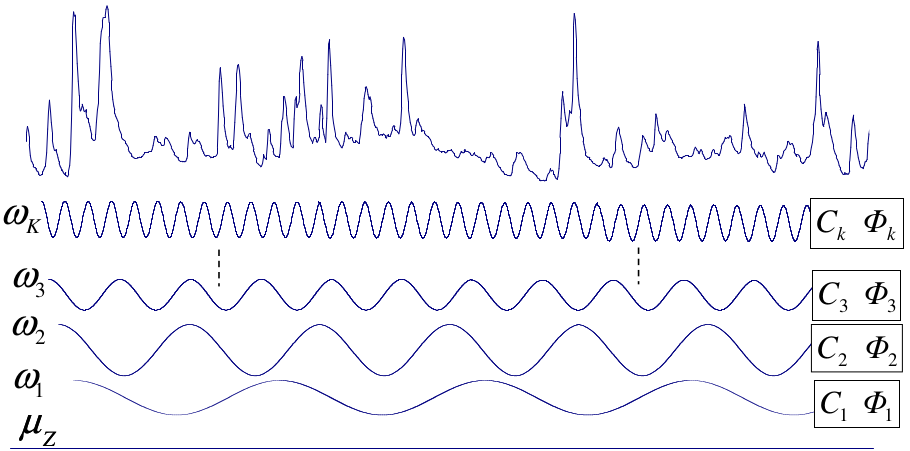
\includegraphics[width=0.9\linewidth]{fiBi510.png}  % from Bierk
    \end{center}
\[
        Z(t) = \mu_Z \pm C_1 \cos(\omega t + \Phi_1) \pm C_2 \cos(2\omega t + \Phi_2) \pm \cdots \pm C_K \cos(K\omega t + \Phi_K)
    \]

\end{frame}

\begin{frame}{Spectral density function}
    Based on the mathematical representation of the spectral decomposition of the random process, the following relationships known as the \alert{Winer-Khinchine relations} are obtained
    \begin{align*}
        C_Z (\tau) &= \int_{-\infty}^{\infty} S_Z(\omega) \cos(\omega \tau) d\omega \\
        S_Z (\omega) &= \frac{1}{2\pi}  \int_{-\infty}^{\infty} C_Z(\tau) \cos(\omega \tau) d\tau 
    \end{align*}
    where the function $S_Z(\omega)$ is known as the \alert{spectral density function} of the \emph{random process}. Note that the equations above show that \emph{covariance function} $C_Z$ is a \alert{Fourier transform} of the \emph{spectrum} and viceversa. These two equations form a \emph{Fourier pair}.  

    Making the lag $\tau = 0$, it is possible to understand the physical meaning of $S_Z (\omega)$ because 
    \[
        C_Z (0) = \int_{-\infty}^{\infty} S_Z(\omega) d\omega
    \]
    from where it can be seen that the \emph{variance} of the random function is equal to the integral over the \emph{spectral density}.This means that the \emph{variance} is a \emph{weighted sum} of variance components, where each component consists of a \emph{random harmonic function} of a given \emph{frequency}.The \emph{spectral density} then represents the weight of each of the attributing \emph{random harmonics}, i.e. the \emph{relative importance} of each \emph{random harmonic} in \emph{explaining} the \emph{total variance} of the \emph{random function}.
\end{frame}

\begin{frame}{Spectral density function}
    It is easy to see the analogy with the \emph{electromagnetic spectrum} where the \emph{total energy} of \emph{electromagnetic radiation} (which is analogous to the variance of our random signal) is found by the \emph{area under the spectrum} and can be attributed to \emph{relative contributions} from different \emph{wavelengths}.
    
    The following table shows expressions for  \emph{spectral density functions} for different \emph{covariance functions}.
    \begin{center}
        \begin{tabular}{|p{3cm}|p{3.8cm}|p{3cm}|}
      Exponential covariance & $C_Z (\tau) = \sigma_Z^2 e^{-|\tau|/a}$ for  $a>0$ & $S_Z (\omega) = \frac{a \sigma_Z^2}{\pi(1+a^2 \omega^2)}$ \\ \hline
      Random harmonic: $Z(t) = a\cos(\omega_0 t + \phi)$ where  $a$ and $\omega_0$ are deterministic constants and $\phi$ is  random. & $C_Z (\tau) = \frac{a^2}{2} \cos(\omega_0 \tau)$  for $\tau \geq 0$ and $a, \omega_0 >0$ & $S_Z (\omega) = \frac{a^2}{4}\delta(\omega-\omega_0)$ \\ \hline
      Hole effect (wave) model & $C_Z (\tau) = \sigma_Z^2 (1-|t|/a)e^{-|\tau|/a}$ for $a>0$ & $S_Z (\omega) = \frac{a^3 \sigma_Z^2 \omega^2}{\pi(1+a^2 \omega^2)^2}$ \\ \hline
      White noise model &  $ \rho_Z (\tau) = \left\{ \begin{array}{l}  1 \text{, if } \tau=0  \\ 0 = \text{, if } \tau>0 \end{array} \right. $ & $S_Z(\omega) = c$\\ 
  \end{tabular}
    \end{center}
 

\end{frame}

\begin{frame}{Spectral density function}
The following figure shows typical realisations of the random functions involved, their correlation function and the associated spectrum.

\begin{minipage}[l]{0.38\textwidth}
    \begin{itemize}
\item Note that the \emph{spectrum} of \emph{white noise} is a \emph{horizontal line}, implying an infinite variance according to the equation. 
\item This shows that \emph{white noise} is a \emph{mathematical construct}, and not a feasible physical process: the \emph{area under the spectrum} is a measure for the \emph{total energy of a process}.
\item  This area is infinitely large, such that all the energy in the universe would not be sufficient to generate such a process.
\item In practice one often talks about \emph{wide band processes}, where the \emph{spectrum} has a \emph{wide band of frequencies}, but encloses a \emph{finite area}.
    \end{itemize}
\end{minipage}
\hfill
\begin{minipage}[l]{0.56\textwidth}
    \begin{center}
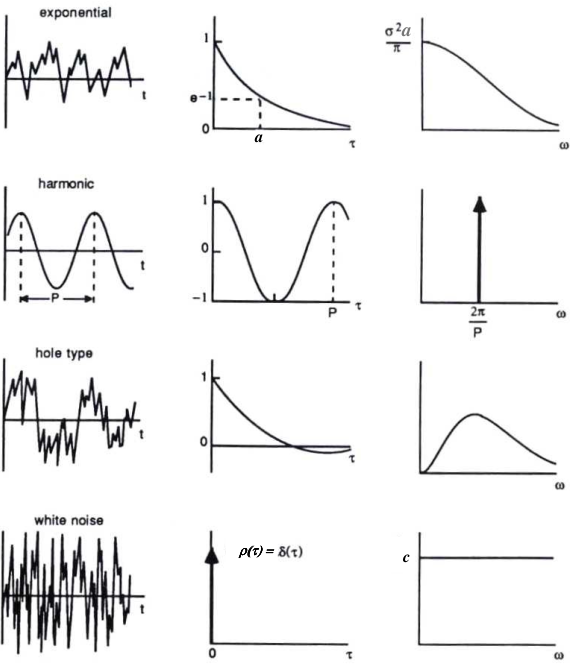
\includegraphics[width=\linewidth]{fiBi511.png}  % from Bierk
    \end{center}
\end{minipage}
\end{frame}

\begin{frame}{Spectral density function}
    Note that \emph{spectral density function} is an even function as the \emph{covariance function}: $S_Z (\omega) = S_Z (-\omega)$. This means that the \emph{spectral density function} can be expressed as a \alert{one-sided function} $G_Z (\omega) = 2 S_Z (\omega)$, for $\omega \geq 0$. The \emph{Wiener-Khinchine relations} become
    \begin{align*}
        C_Z (\tau) &= \int_0^{\infty} G_Z(\omega) \cos(\omega \tau) d\omega \\
        G_Z (\omega) &= \frac{2}{\pi} \int_0^{\infty} C_Z(\tau) \cos(\omega \tau) d\omega \\
    \end{align*}
    Sometimes it is convenient to work with the \emph{normalised spectral density functions}, by dividing the \emph{spectra} by the \emph{variance}: $s_Z (\omega) = \frac{S_Z (\omega)}{\sigma_Z^2}$ and $g_Z (\omega) = \frac{G_Z (\omega)}{\sigma_Z^2}$. There is a relation between the \emph{normalised spectral density function} $s_Z(\omega)$ and the scale of fluctuation. So if $\omega=0$ we obtain
    \[
        s_z (0) = \frac{1}{2\pi} \int_{-\infty}^{\infty} \rho_Z (\tau) d\omega = \frac{\theta}{2\pi}
    \]

\end{frame}

\begin{frame}{Formal spectral representation}
    A more formal representation of the \emph{spectral density} is used in the literature based on \emph{complex calculus}. Here the random function $Z(t)$ is defined as the \emph{real part $Re{.}$}   of a \emph{complex random function} $Z^* (t)$.   
\[
    Z(t) = Re\{Z^* (t)\} = Re \left\{ \mu_Z + \sum_{k=-K}^{K} X_k e^{i\omega_k t} \right\} \xrightarrow[K \rightarrow \infty]{} Re\left\{ \mu_Z + \int_{-\infty}^{\infty} e^{i\omega t} dX (\omega) \right\} 
\]
where $\omega_k = \frac{1}{2} (2k-1) \Delta \omega$ is the frequency, and $X_k$ a \emph{random complex number} representing the \emph{amplitude}.  This equation means that the \emph{complex random process} is decomposed into a large number of complex harmonic functions $e^{i\omega t} = \cos(\omega t) + i\sin(\omega t)$ with  \emph{random complex amplitude}. According to this representation, the \emph{Wiener-Khinchine} equations are
    \begin{align*}
        C_Z (\tau) &= \int_{-\infty}^{\infty} S_Z(\omega) e^{i\omega \tau}  d\omega \\
        S_Z (\omega) &= \frac{1}{2\pi} \int_{-\infty}^{\infty} C_Z(\tau)^{i\omega \tau} d\tau \\
    \end{align*}
    It can be demonstrated that these equations are equivalent to the prior \emph{Wiener-Khinchine} the equations. 
\end{frame}

\begin{frame}{Estimating the spectral density function}
    For \emph{stationary  random functions}, the \emph{spectral density function} can be estimated from the \emph{covariance function} as
    \[
        S_Z (\omega_i) = \frac{1}{2\pi} \left(\lambda_0 C_Z(0) + 2 \sum_{k=1}^M \lambda_k \hat{C}_Z (k\Delta \tau) \cos(\omega_i k)  \right)
        \]
        where $\omega_i = i\pi/M$ and $|i| = 1, 2, \cdots, M$. The weights $\lambda_k$ are necessary to smooth the covariances before performing the transformation. So that, a smooth \emph{spectral density function} is obtained displaying only the relevant features. There are numerous ways to estimate the \emph{smoothing weights}, the most common are:
        \begin{itemize}
            \item \alert{Tukey window}

                \[
                    \lambda_k = \frac{1}{2} \left( 1 + \cos\left(\frac{k\pi}{M}\right) \right), \quad \quad k=1, 2, \cdots, M
                \]

            \item \alert{Parzen window}
                \[
\lambda_k = 
\left\{
\begin{array}{l}
                   1-6\left( \frac{k}{M} \right)^2 + 6\left( \frac{k}{M} \right)^3, \quad \quad 0\leq k \leq M/2 \\ \\
                   \left(2-\frac{k}{m}\right)^3, \quad \quad M/2 \leq k \leq M
\end{array}
\right.
                \]
        \end{itemize} 
        The \emph{highest frequency} that is analysed is equal  to $f_{max} = \frac{\omega_{max}}{2\pi} = 0.5$, which is the \emph{highest frequency} that can be estimated from a time series: half of the frequency of the observations. This frequency is called the \alert{Nyquist frequency}.  For instance, if streamflow is observed once per day, the highest frequency that can be detected is on cycle per two days. 
\end{frame}

\begin{frame}{Estimating the spectral density function}
The \emph{smallest frequency} (largest wavelength) that can be analysed depends on the discretisation $f_{min} = \pi/(2\pi M) = 1/2 M$, where $M$ is the cutoff level (maximum lag considered) of the covariance function. The width of the \emph{smoothing windows} (smoothing weight) is adjusted accordingly.

The figure below shows the spectrum of a daily discharge time series. The \emph{spectral density function} was estimated using a \emph{Parzen window} with $M=9000$. Clearly, small frequencies dominate with a small peak between 4 and 5 years. Most prominent of course, as expected, there is a peak at a frequency of once a year, which exemplifies the strong seasonality in the time series.
    \begin{center}
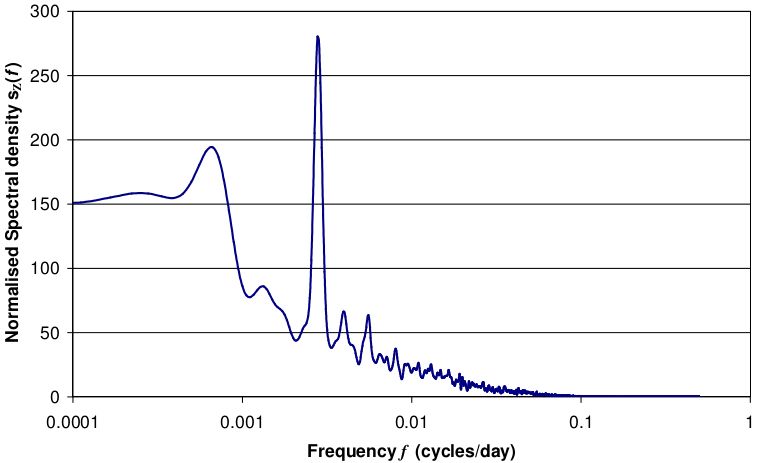
\includegraphics[width=0.8\linewidth]{fiBi512.png}  % from Bierk
    \end{center}
\end{frame}

\begin{frame}{Spectral representations of random space functions}
    Extending the equations above to two dimensions, the \emph{stationary random function} $Z(x_1, x_2)$ can be expressed  in terms of random harmonics as
    \[
        Z(x_1, x_2) = \mu_Z + \sum_{k_1 = -K_1}^{k_1 = K_1}  \sum_{k_2 = -K_2}^{k_2 = K_2} C_{12} \cos(\omega_{k_1} x_1 + \omega_{k_2} x_2 + \Phi_{12})
    \]
    where $C_{12}$ and $\Phi_{12}$ are the \emph{random amplitude} and the \emph{phase angle}, respectively, belonging to frequency $\omega_{k_i}$, $i=1,2$ 
    \[
        \omega_{k_i} = \pm \frac{2 k_i \Delta \omega_i -1}{2}
    \]

    The \emph{Wiener-Khinchine} equations then become
    \begin{align*}
        C_Z (h_1, h_2) &= \int_{-\infty}^{\infty} \int_{-\infty}^{\infty} S_Z(\omega_1, \omega_2) \cos(\omega_1 h_1 + \omega_2 h_2) d\omega_1 d\omega_2 \\
        S_Z (\omega_1, \omega_2) &= \frac{1}{(2\pi)^2} \int_{-\infty}^{\infty} \int_{-\infty}^{\infty} C_Z(h_1, h_2) \cos(\omega_1 h_1 + \omega_2 h_2) d\omega_1 d\omega_2 \\
    \end{align*}
    The \emph{variance} is given by the volume under the \emph{2D spectral density function} $S_Z (\omega_1, \omega_2)$. Therefore
    \[
        \sigma_Z^2 = \int_{-\infty}^{\infty} \int_{-\infty}^{\infty} S_Z(\omega_1, \omega_2)  d\omega_1 d\omega_2 
    \]
\end{frame}

%-------
% From Bierke
\section{Local averaging of stationary random functions}
\begin{frame}{Local averaging of stationary random functions}
    For a \emph{stationary random function} $Z(t)$, the \emph{local moving averaging function} $Z_T (t)$ of $Z(t)$ is defined as
    \[
        Z_T (t) = \frac{1}{T}\int_{t-T/2}^{t+T/2} Z(\tau) d\tau
    \]
    The figure below shows the \emph{Local (moving) averaging} of a \emph{stationary random function}.
    \begin{center}
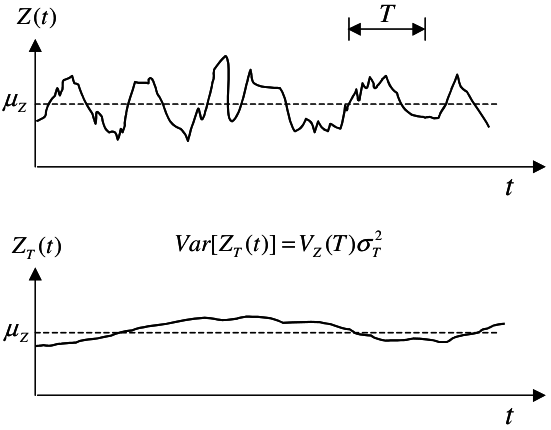
\includegraphics[width=0.8\linewidth]{fiBi513.png}  % from Bierk
    \end{center}

\end{frame}

\begin{frame}{Local averaging of stationary random functions}
    Note that \emph{local averaging} of a \emph{stationary random process} will not affect the \emph{mean}, but it does reduce the \emph{variance}. So the \emph{variance} of the \emph{averaged process}  $Var[Z_T (t)] = E\left[(Z_T (t) - \mu_Z)^2\right]$ can be calculated for $\mu_Z  = 0$ as

\[
    \begin{aligned}
        Var[ Z_T (t) ] &= E\left[ \frac{1}{T}\int_{t-T/2}^{t+T/2} Z(\tau_1) d\tau_1 \frac{1}{T}\int_{t-T/2}^{t+T/2} Z(\tau_2) d\tau_2 \right] \\
                      &= E\left[ \frac{1}{T}\int_{0}^{T} Z(\tau_1) d\tau_1 \frac{1}{T}\int_{0}^{T} Z(\tau_2) d\tau_2 \right] \\
                      &= \frac{1}{T^2} \int_{0}^{T} \int_{0}^{T} E\left[ Z(\tau_1) Z(\tau_2) \right] d\tau_1 d\tau_2 \\
                      &= \frac{1}{T^2} \int_{0}^{T} \int_{0}^{T} C_Z (\tau_2 - \tau_1) d\tau_1 d\tau_2 
    \end{aligned}
\]
From $Var[ Z_T (t) ]$ a new function is introduced called the \alert{variance function}
\[
    V_Z (T) = \frac{Var[Z_T (t)]}{\sigma_Z^2}
\]
The \emph{variance function} thus describes the reduction in variance when averaging a random function as a function of the \emph{averaging interval T}.
\end{frame}

\begin{frame}{Local averaging of stationary random functions}
    The \emph{variance function} is related to the \emph{correlation function} as
    \[
        V_Z (t) = \frac{1}{T^2} \int_{0}^{T} \int_{0}^{T} \rho_Z (\tau_2 - \tau_1) d\tau_1 d\tau_2 
    \]
This equation can be simplified as
\[
    V_Z (t) = \frac{1}{T} \int_{0}^{T} \left( 1- \frac{\tau}{T} \right) \rho_Z (\tau) d\tau
\]

The table below gives a number of \emph{correlation functions} and their \emph{variance functions}. 

    \begin{center}
        \begin{tabular}{|p{2cm}|p{3cm}|p{5.2cm}|}
  Exponential (first order autoregressive process) & $\rho_z (\tau) =  e^{-\tau/a}$ for $\tau \geq 0$, $a>0$ & $V(T) = 2 \left(\frac{a}{2}\right)^2 \left(\frac{T}{a} -1 + e^{-T/a} \right)$ $\theta = 2a$\\ \hline
  Second order autoregressive process & $\rho_z (\tau) = \left[ 1 + \frac{\tau}{a}\right] e^{-\tau/a}$  for $\tau \geq 0$, $a>0$ & $V(T) = \frac{2a}{T} \left[2 + e^{-T/a} - \frac{2a}{T} \left(1- e^{-T/a} \right) \right]$ $\theta = 4a$ \\ \hline
  Gaussian correlation function & $\rho_z (\tau) =  e^{-\tau^2 /a^2 }$  for $\tau \geq 0$, $a>0$ & $V(T) = \left(\frac{a}{T}\right)^2 \left[\sqrt{\pi} Erf\left(\frac{T}{a}\right) -1  + e^{-T^2/a^2}\right]$ $\theta = a\sqrt{\pi}$  
  \end{tabular}
    \end{center}
    where $\tau = |t_2 - t_1|$. 

\end{frame}

\begin{frame}{Local averaging of stationary random functions}
    If we analysed the \emph{variance function} when $T \rightarrow \infty$, $\lim_{T\rightarrow \infty} V_Z (T) \rightarrow \frac{\theta}{T}$, where $\theta$ is the \alert{scale of fluctuation}. The \emph{scale of fluctuation} is also given for the three correlation models given in the table above. The \emph{scale of fluctuation} was already introduced earlier as a measure of \emph{spatial correlation} of the \emph{random function} and can also be calculated using the \emph{correlation function } or the \emph{spectral density}. 

    $V_Z (T) \rightarrow \frac{\theta}{T}$ states that for larger averaging intervals the variance reduction through averaging is inversely proportional to the \emph{scale of fluctuation}: the larger the \emph{scale of fluctuation} the larger $T$ should be to achieve a given variance reduction.

    The \emph{covariance} of the averaged  process is given by
    \[
        C_Z (T, \tau^2) =\frac{1}{T^2} \int_0^{T} \int_0^{\tau + T} C_Z (t_1, t_2) dt_1 dt_2
    \]
    This equation is usually solved by the implementation of \emph{numerical integration}. 

    In the case of \emph{2D random fields} (in space where $\mathbf{x} = {x,y}$), the local average process is over an area $A=L_1 L_2$ and is defined as
    \[
        Z_T (x_1, x_2) =\frac{1}{L_1 L_2} \int_{x_1 - L_1/2 }^{x_1 + L_1/2} \int_{x_2 - L_2/2 }^{x_2 + L_2/2} Z(u_1, u_2) du_1 du_2
    \]
     
\end{frame}

\begin{frame}{Local averaging of stationary random functions}
    The \emph{variance function} is given by
    \[
        V_Z (L_1, L_2) =\frac{1}{L_1 L_2} \int_{0}^{L_1} \int_{0}^{ L_2} \left(1- \frac{h_1}{L_1} \right) \left(1- \frac{h_2}{L_2} \right) \rho_Z (h_1, h_2) dh_1 dh_2
    \]
    The limit of the \emph{variance function} defines the spatial \alert{scale of fluctuation} or \alert{characteristic area}
    \[
        \lim_{L_1, L_2 \rightarrow \infty} V_Z (L_1, L_2) \rightarrow \frac{\alpha}{L_1 L_2}
    \]
    where
    \[
        \alpha = \int_{-\infty}^{\infty} \int_{-\infty}^{\infty} \rho_Z (u_1, u_2) du_1 du_2
    \]
    The \emph{characteristic area $\alpha$} can also be obtained through the spectral representation  by setting $\omega_1 = \omega_2 = 0$ in the \emph{Wiener-Khinchine relation}, so
    \[
        s_Z (0,0) = \frac{S_Z (0,0)}{\sigma_Z^2} = \frac{1}{4\pi^2}\int_{-\infty}^{\infty} \int_{-\infty}^{\infty}  \rho_Z (h_1, h_2) dh_1 dh_2
    \] 

    combining the two last equations
    \[
        \alpha = 4 \pi^2 s_z(0,0)
    \]

\end{frame}

\begin{frame}{Local averaging of stationary random functions}
    The \emph{covariance} of the \emph{averaged random field} in 2D is given by
    \[
        C_Z (L_1, L_2; h_1, h_2) = \frac{1}{(L_1 L_2)^2} \int_{0}^{L_1}\int_{0}^{L_2}\int_{h_1}^{L_1 + h_1}\int_{h_2}^{L_2 + h_2} C_Z ( x_1, y_1, x_2, y_2) dx_1 dy_1 dx_2 dy_2
    \]

    The \emph{covariance} of the \emph{spatially averaged random function} is frequently used in \emph{geostatistical mapping}, where its values are approximated with \emph{numerical integration}. In vector notation where $\mathbf{x_1} = (x_1, y_1)^T$, $\mathbf{x_2} = (x_2, y_2)^T$, $\mathbf{h} = (h_1, h_2)^T$ and $A= L_1 L_2$
    \[
        C_Z (A, \mathbf{h}) = \frac{1}{A^2} \int_A \int_{A+\mathbf{h}} C_Z (\mathbf{x_1}, \mathbf{x_2}) d\mathbf{x_1} d\mathbf{x_2} 
    \]


\end{frame}
\end{document}
